\chapter{Aspectos generales de las estrellas de neutrones}

Como se mencionó en la introducción, las estrellas han sido estudiadas extensivamente durante 50 años y a pesar de que sus más importantes características no han sido predichas unívocamente ($M_{\text{max}}$ y $R_{1.4}$), debido a su sensible dependencia de la EOS de la materia nuclear ultradensa,%al reto teórico que representa obtenerla a partir de una teoría relativista de muchos cuerpos para partículas que interactúan fuertemente,
la EOS en regiones con densidades menores a $\rho_0$ se conocen con la suficiente precisión \cite{Haensel2007,Chamel2008} para reconocer características generales de su estructura interna. 

En este capítulo se resumirá el conocimiento actual de las estrellas de neutrones comenzando por cómo son formadas, describiendo las regiones interiores que se conocen relativamente bien y mencionando las hipótesis respecto a la composición de su núcleo. Finalmente se presentarán algunas de las manifestaciones observacionales más importantes de las estrellas de neutrones.


\section{De estrellas normales a estrellas de neutrones}

Las estrellas son formadas a partir de nubes de gas interestelar, compuestas en su mayoría de hidrógeno molecular, que debido a algún tipo de perturbación comienzan a colapsar gravitacionalmente. La compresión del gas incrementa su temperatura hasta que la presión es capaz de balancearla, alcanzando el equilibrio hidrostático. Este equilibrio dura poco debido a que la pérdida de energía (en forma de radiación) disminuye la temperatura del gas y la consecuente reducción de la presión permite que la contracción continúe. El proceso de contracción y equilibrio del material se repite durante un periodo de tiempo (fase pre-secuencia principal), hasta que la temperatura aumenta lo suficiente para que la fusión de hidrógeno en helio pueda ocurrir en el núcleo ($T\approx 10^7\,\si{\kelvin}$). Este proceso de fusión nuclear compensa las pérdidas radiativas y mantiene a la estrella en un equilibrio hidrostático estable \cite{Scilla2016}.

Las reacciones nucleares pueden sostener a la estrella durante la mayor parte de su vida luminosa (de millones a billones de años, dependiendo de su masa inicial \cite{Salaris2005}). Estrellas en esta fase forman la secuencia principal del diagrama de Hertzsprung-Russell.
\setcounter{footnote}{0}
\begin{figure}[H]
    \centering
    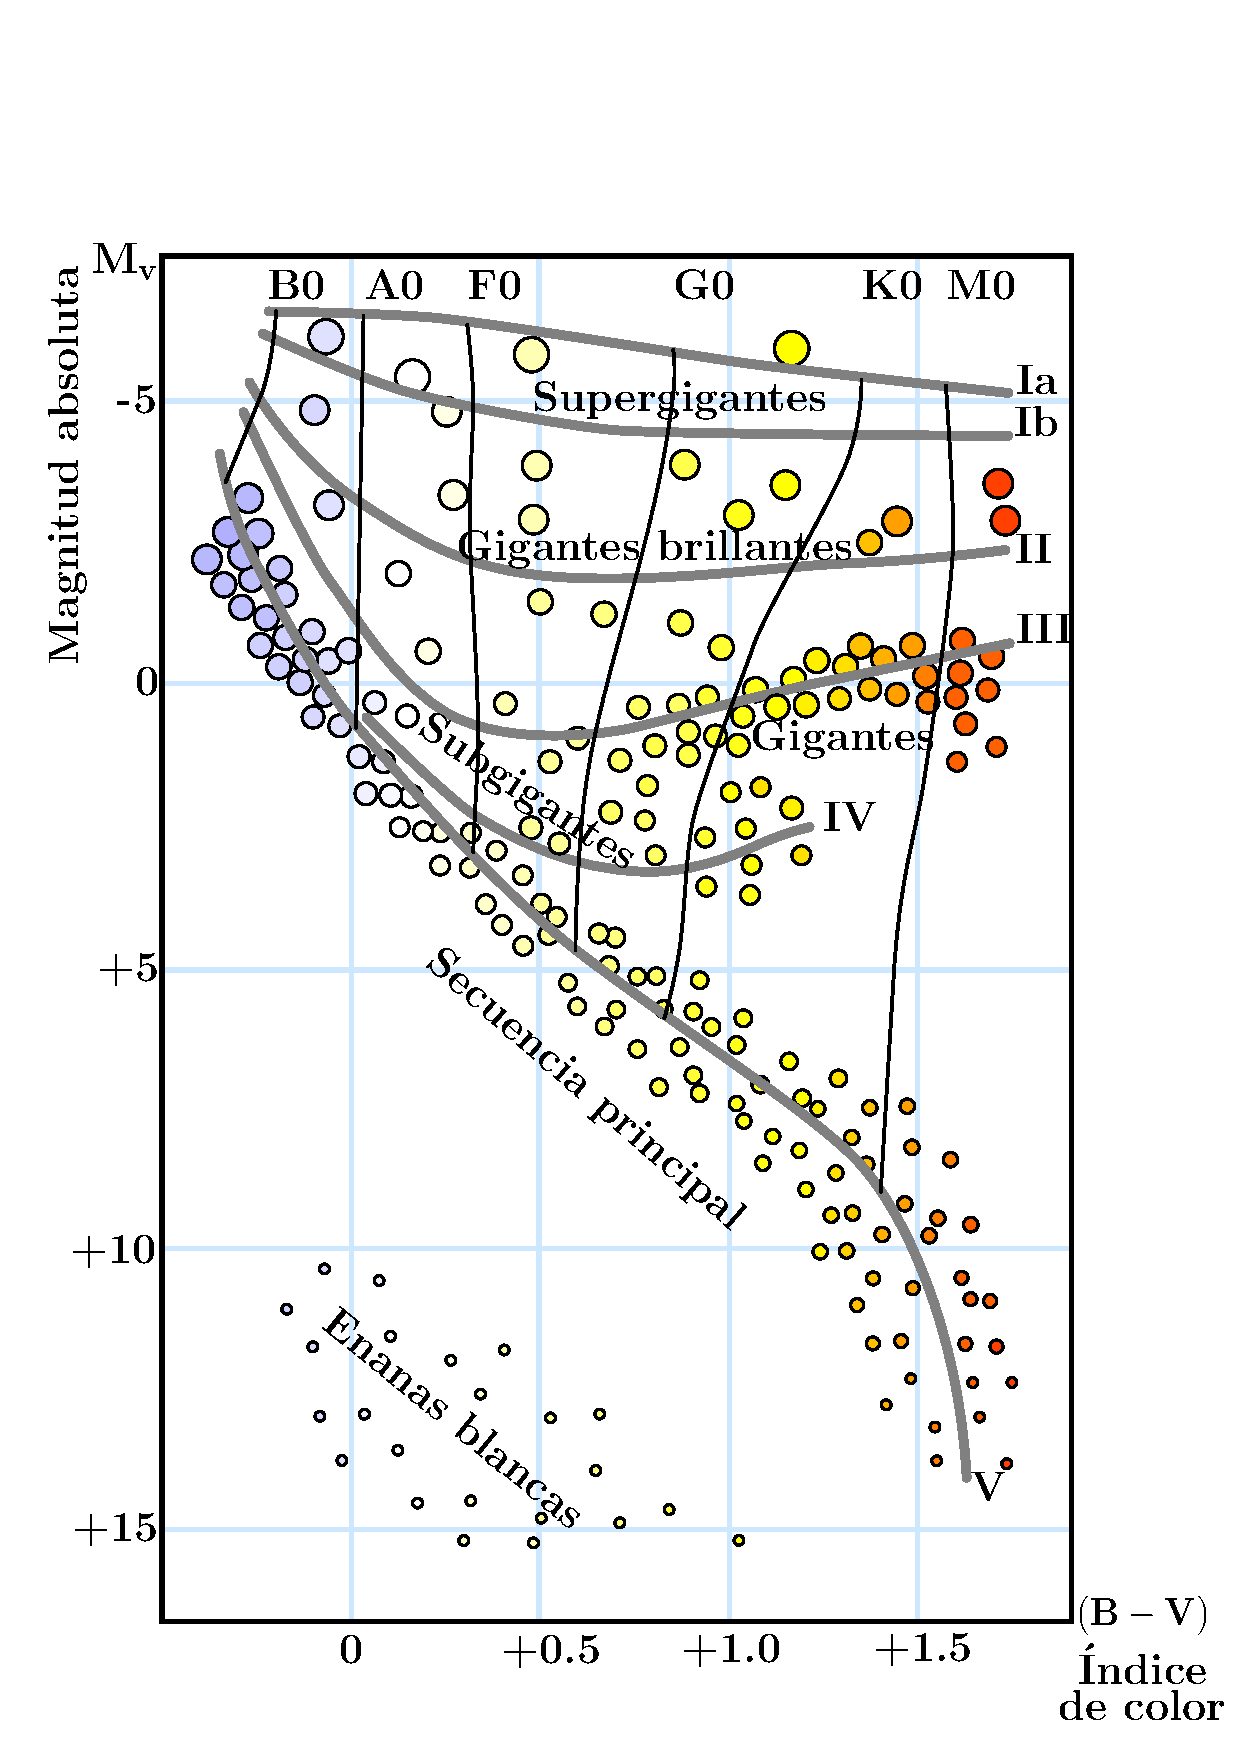
\includegraphics[width=205pt]{figures/H-R_diagram.pdf}%
    \caption[Diagrama Hertzsprung-Russell]{Diagrama Hertzsprung-Russell.\protect\footnotemark}
    \label{HR}
\end{figure}
\footnotetext{Adaptado de \url{https://commons.wikimedia.org/wiki/File:H-R_diagram.svg}}

La evolución de la estrella después de agotar el hidrógeno depende de su masa: estrellas con \emph{masas pequeñas e intermedias} ($M\leq M_{\odot}$) procederán a fusionar helio formando carbono en su núcleo. Esto representa una transición de la secuencia principal hacia la rama de gigantes (hacia el rojo) en el diagrama de Hertzsprung-Russell. Durante las últimas etapas de evolución, estas estrellas liberan sus capas más externas formando una nebulosa planetaria y dejando un núcleo que será sostenido por la presión de degeneración de electrones, conocido como una enana blanca \cite{Padmanabhan2000}.

Estrellas \emph{masivas} ($M>8 M_{\odot}$) entran en un ciclo de fusión de elementos en su núcleo, formando elementos cada vez más pesados (helio, carbono, oxígeno, magnesio, silicio y hierro) \cite{Glendenning2000}. Al final de cada una de estas etapas de fusión los elementos pesados recién creados formarán un núcleo, y los restos del elemento ligero forman un cascarón a su alrededor. En el diagrama de Hertzsprung-Rusell estas estrellas llegarán hasta la parte superior de la secuencia principal y se moverán hacia la rama de supergigantes. Al alcanzar el hierro, la fusión deja de ser exotérmica (en vez de liberar energía la requerirá) y deja a la estrella sin una fuente de energía que mantenga el equilibrio hidrostático. Estas estrellas colapsarán eventualmente en un evento conocido como supernova (tipo II)\cmmt{ de colapso de núcleo}: los cascarones de los distintos elementos caen sobre el núcleo de hierro desencadenando, mediante mecanismos que no han sido enteramente comprendidos \cite{Janka2012}, la eyección de gran parte de su masa en una explosión \cite{Woosley2005}.

Tras la supernova, el núcleo colapsado \cmmt{ —cuya composición precisa no se conoce pero se presume contiene neutrones, protones, mesones, hiperones e incluso quarks desconfinados—}  inicia un proceso de enfriamiento y reajuste estructural, durante el cual emite una gran cantidad de energía en forma de radiación y neutrinos (importantes a la hora de verificar modelos teóricos, cf. \cite{Alvarez-Salazar2018}). Después de alcanzar una composición estable —no conocida con precisión pero se presume contiene neutrones, protones, mesones, hiperones e incluso quarks desconfinados \cite{Lattimer2004}— la presión de degeneración de sus componentes y la repulsión de rango corto entre nucleones sostendrán el núcleo colapsado \cite{Glendenning2000}, alcanzando una estructura definida conocida generalmente como un objeto compacto o estrella de neutrones.

\section{Estructura interna}
La composición de las estrellas de neutrones, contrario a lo que el nombre sugiere, se presume es muy rica y varía a lo largo de su extensión radial, esta variada composición y las distintas fases que exhiben, están distribuidas en una estructura de cascarones, denominada generalmente una red cristalina de Coulomb (ver Figura \ref{NSC}).
La superficie de la estrella está rodeada por una \emph{atmósfera} compuesta principalmente de hidrógeno, helio y hierro en estado gaseoso o condensado dependiendo de su temperatura superficial y campo magnético \cite{Zavlin2002}. % La atmósfera es importante porque es donde se forma el espectro de radiación electromagnética y éste aporta información acerca de su composición, temperatura y campo magnético.
Bajo la atmósfera se encuentra una \emph{envoltura} (de aproximadamente 100 \si{\metre}), a veces llamado océano. Compuesta presuntamente de núcleos alrededor del pico del hierro en un estado condensado, la envoltura influencia el transporte y emisión de energía térmica desde la superficie \cite{Piekarewicz2013,Potekhin2010,Lattimer2004}.

La envoltura encierra a cuatro regiones internas: la corteza exterior e interior y el núcleo exterior e interior. La \emph{corteza} es una capa en la que se encuentra materia con densidades sub-nucleares ($\rho < \rho_0$). En la \emph{corteza exterior} los electrones presentes, requeridos para la neutralidad de carga de la estrella, forman un gas de Fermi y ocurre un proceso de neutronización donde los electrones son capturados por protones para crear neutrones. La división con la \emph{corteza interior} se presenta debido a que a una densidad $\rho_{ND}\simeq 10^{11}\, \si{\gram\per\centi\metre^2}$ (neutron drip density), los neutrones comienzan a \com{gotear} del núcleo, por lo que hay presencia de neutrones libres, que pueden llegar a condensarse en un superfluido \cite{Baldo2005}. En el fondo de la corteza, cuando la densidad se acerca a $\rho_0$, se ha predicho la presencia de fases conocidas como \com{pasta} nuclear, en las que, debido a la compresión, los núcleos se deforman y dejan de ser esféricos (para una revisión de la corteza de las estrellas de neutrones consultar la referencia \cite{Chamel2008} y referencias allí citadas). 

\begin{figure}[H]
    \centering
    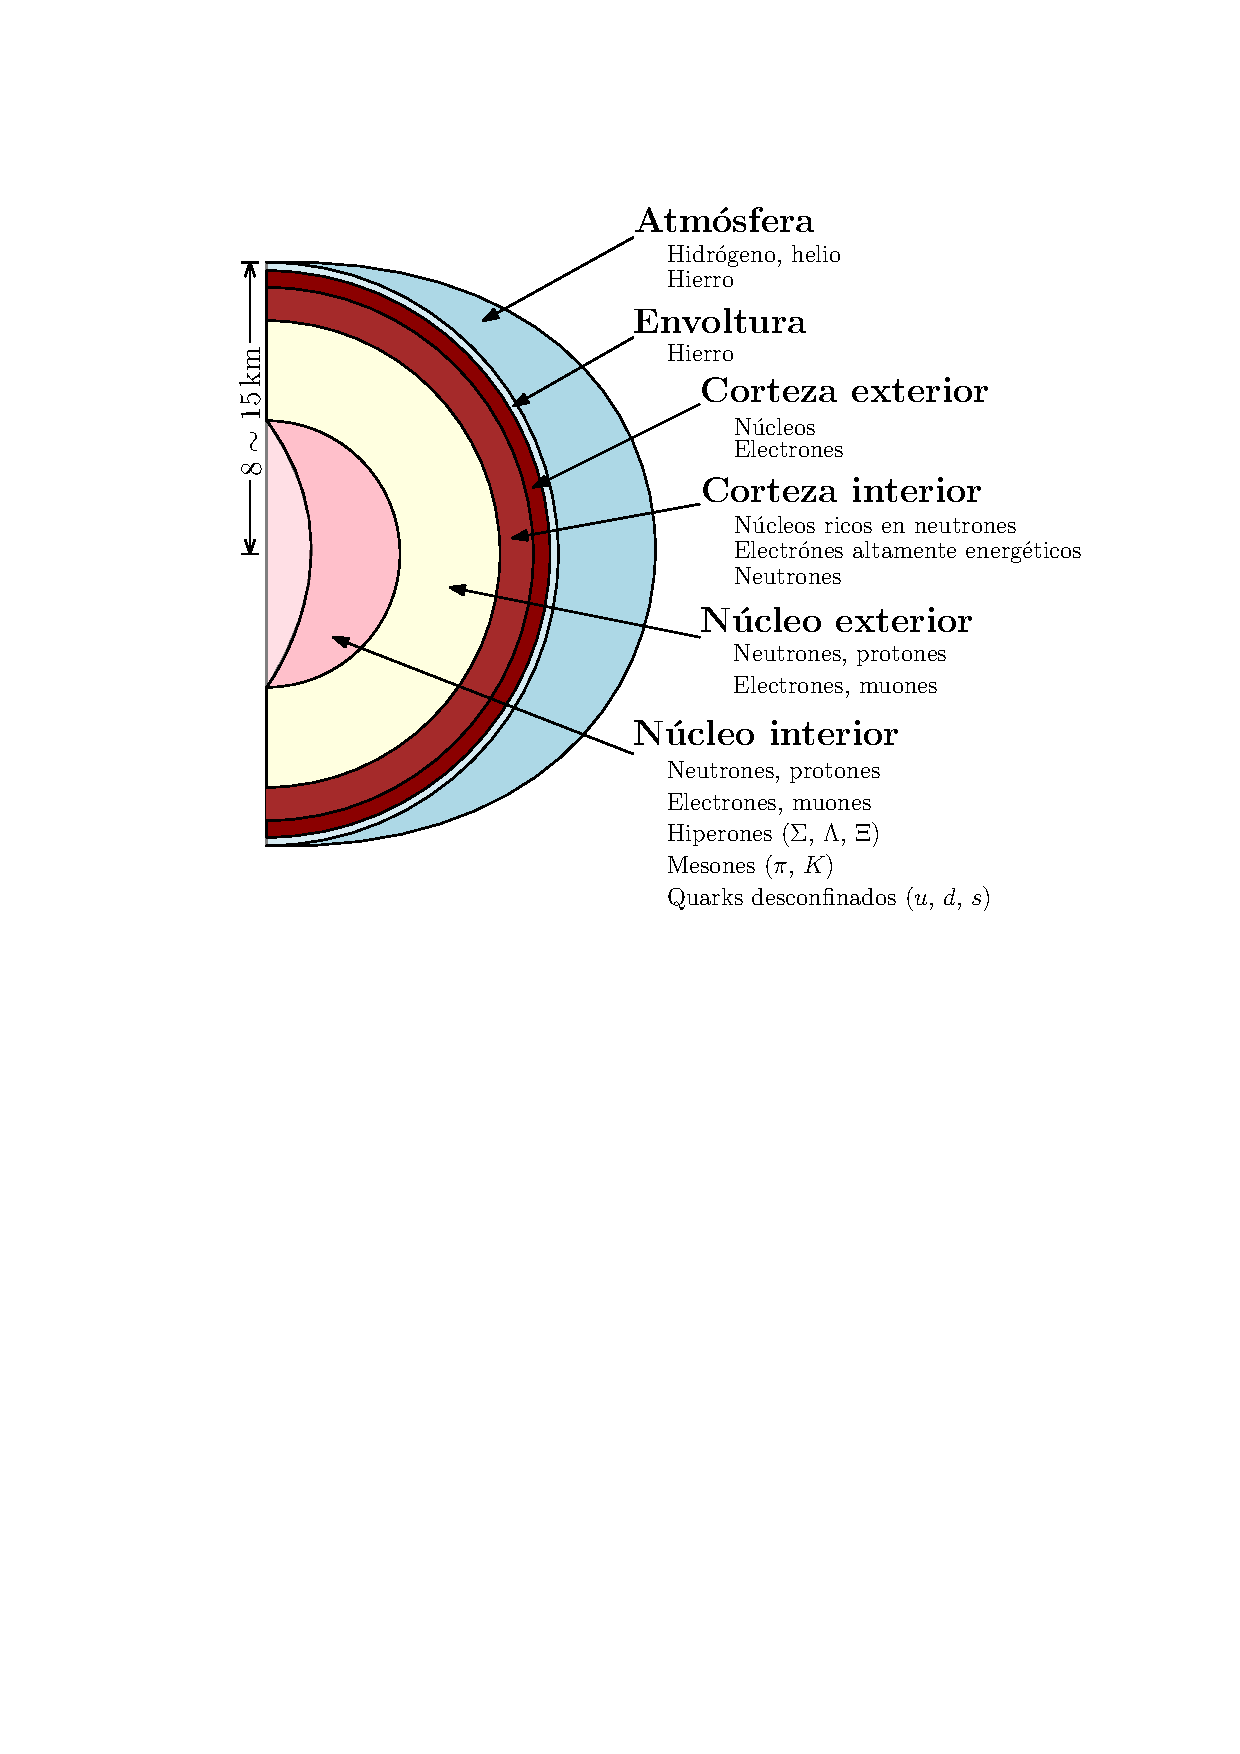
\includegraphics[width=300pt]{figures/neutronstar.pdf}
    \caption{Composición de una estrella de neutrones.\protect\footnotemark}
    \label{NSC}
\end{figure}
\footnotetext{Adaptado de \cite{Weber2012}, Figura 1.}


El \emph{núcleo} comprende regiones en las que la densidad alcanza $\rho_0$ y contiene la mayor fracción de la masa estelar. Está subdividido un dos: el \emph{núcleo exterior}, con densidad $\num{0.5}\rho_0\lesssim\rho\lesssim 2\rho_0$  cuya composición se conoce bien cualitativamente \cite{Haensel2007}: es un superfluido de neutrones y protones, con presencia de electrones y muones altamente degenerados. Del \emph{núcleo interior}, por el contrario, no se conoce su composición. Se ha sugerido la presencia de hiperones, piones, kaones e incluso quarks desconfinados (consultar las revisiones \cite{Potekhin2010,Lattimer2004} y referencias allí citadas).



\begin{figure}[H]
    \centering
    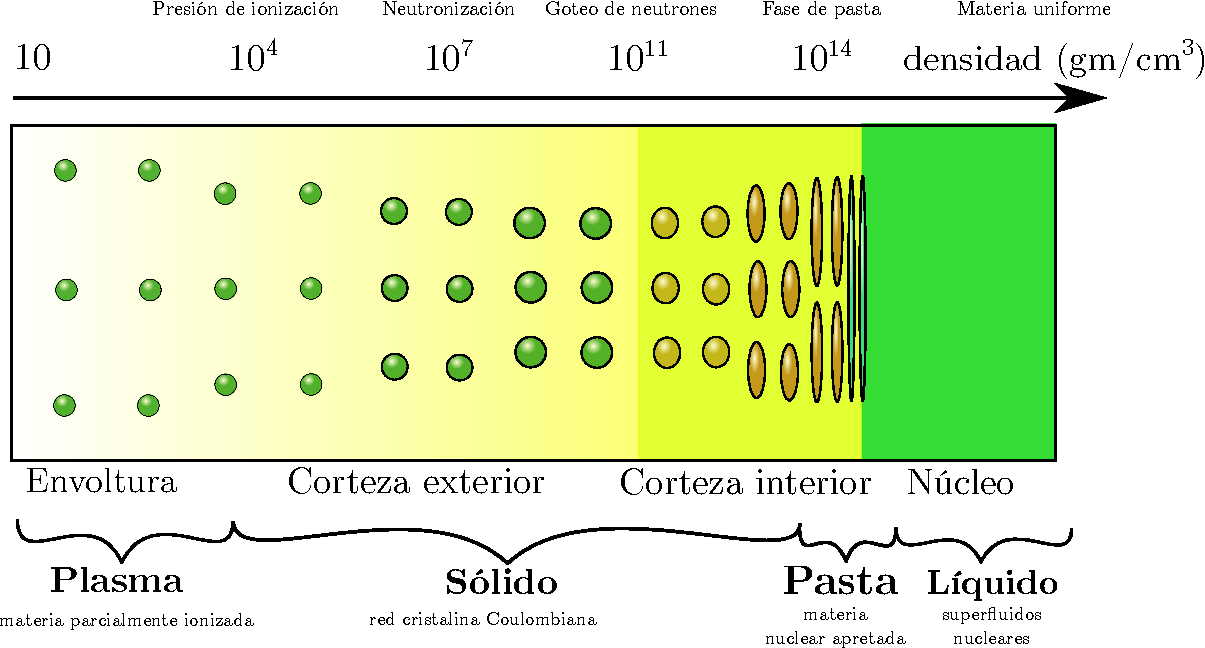
\includegraphics[width=420pt]{figures/Density.pdf}
    \caption[Estructura interna de una estrella de neutrones]{Estructura interna de una estrella de neutrones.\protect\footnotemark}
    \label{NSS}
\end{figure}
\footnotetext{Adaptado de \cite{Chamel2008}, Figura 4.}   


\section{Observaciones}

La gran variedad de manifestaciones observacionales de las estrellas de neutrones les permite ser observadas no solo en todas las bandas del espectro electromagnético, sino en los eventos de ondas gravitacionales. En esta sección se discutirá brevemente dos de sus principales manifestaciones: los pulsares y la radiación térmica, comúnmente usadas para medir masas y radios, respectivamente.

\subsection{Pulsares}

Los pulsares son estrellas de neutrones magnetizadas que rotan rápidamente emitiendo radiación desde la magnetósfera, orientada principalmente en los polos magnéticos, a expensas de su energía rotacional \cite{Becker2009}, estos son detectados cuando uno de estos rayos cruza la tierra. La mayoría de las estrellas de neutrones conocidas son observadas como pulsares con un espectro en el rango del radio. Aunque la mayoría de pulsares de radio están aislados, una pequeña cantidad de pulsares pertenecen a sistemas binarios los cuales son de suma importancia pues todos los métodos para medir la masa de los pulsares están basados en el trazado del movimiento orbital del sistema usando el tiempo de llegada de los pulsos observados \cite{Ozel2016}.

\TODO{Quizá listar los métodos que usan a los pulsares}

\subsection{Emisión térmica}

Una parte apreciable de la radiación emitida por estrellas de neutrones aisladas parece ser radiación térmica originada cerca a su superficie. Esta radiación es emitida principalmente en las rayos X blandos.

\TODO{Listar métodos que usan radiación térmica para medir el radio}

Recientemente se ha identificado que las curvas de enfriamiento, dependencia temporal de la luminosidad detectada por un observador lejano, proveen una manera de caracterizar la estructura interna de las estrellas \cite{Yakovlev2004}.

